%% LyX 2.1.4 created this file.  For more info, see http://www.lyx.org/.
%% Do not edit unless you really know what you are doing.
\documentclass{beamer}
\usepackage{hyperref}
%\usepackage{minted}
\usepackage{animate}
\usepackage{graphicx}
\def\Put(#1,#2)#3{\leavevmode\makebox(0,0){\put(#1,#2){#3}}}
\usepackage{color}
\usepackage{tikz}
\usepackage{amssymb}
\usepackage{enumerate}

\newcommand\blfootnote[1]{%
  \begingroup
  \renewcommand\thefootnote{}\footnote{#1}%
  \addtocounter{footnote}{-1}%
  \endgroup
}

\definecolor{LightGray}{gray}{0.9}

\ifx\hypersetup\undefined
  \AtBeginDocument{%
    \hypersetup{unicode=true,
 bookmarksnumbered=false,bookmarksopen=false,
 breaklinks=false,pdfborder={0 0 0},colorlinks=false}
  }
\else
  \hypersetup{unicode=true,
 bookmarksnumbered=false,bookmarksopen=false,
 breaklinks=false,pdfborder={0 0 0},colorlinks=false}
\fi

\makeatletter
%%%%%%%%%%%%%%%%%%%%%%%%%%%%%% Textclass specific LaTeX commands.
 % this default might be overridden by plain title style
 \newcommand\makebeamertitle{\frame{\maketitle}}%
 % (ERT) argument for the TOC
 \AtBeginDocument{%
   \let\origtableofcontents=\tableofcontents
   \def\tableofcontents{\@ifnextchar[{\origtableofcontents}{\gobbletableofcontents}}
   \def\gobbletableofcontents#1{\origtableofcontents}
 }

%%%%%%%%%%%%%%%%%%%%%%%%%%%%%% User specified LaTeX commands.
\usetheme{Malmoe}
% or ...
\useoutertheme{infolines}
\addtobeamertemplate{headline}{}{\vskip2pt}

\setbeamercovered{transparent}
% or whatever (possibly just delete it)



\setbeamertemplate{footline}
{
  \leavevmode%
  \hbox{%
  \begin{beamercolorbox}[wd=.5\paperwidth,ht=2.25ex,dp=1ex,center]{title in head/foot}%
    \usebeamerfont{title in head/foot}\insertshorttitle
  \end{beamercolorbox}%
  \begin{beamercolorbox}[wd=.5\paperwidth,ht=2.25ex,dp=1ex,right]{date in head/foot}%
    \usebeamerfont{date in head/foot}\insertshortdate{}\hspace*{2em}
    \insertframenumber{} / \inserttotalframenumber\hspace*{2ex} 
  \end{beamercolorbox}}%
  \vskip0pt%
}

\makeatother

\begin{document}

\title[Discussion 3 - Modular Arithmetic]{CS/MATH 111, Discrete Structures - Fall 2018. \\ Discussion 3 - Modular Arithmetic }
\author{Andres, Sara, Elena}
\institute{University of California, Riverside}

\makebeamertitle

% \AtBeginSection[]{
%   \frame<beamer>{ 
%     \frametitle{Agenda}   
%     \tableofcontents[currentsubsection] 
%   }
% }

\newif\iflattersubsect

\AtBeginSection[] {
    \begin{frame}<beamer>
    \frametitle{Outline} %
    \tableofcontents[currentsection]  
    \end{frame}
    \lattersubsectfalse
}

\AtBeginSubsection[] {
    % \iflattersubsect
    \begin{frame}<beamer>
    \frametitle{Outline} %
    \tableofcontents[currentsubsection]  
    \end{frame}
    % \fi
    % \lattersubsecttrue
}

\section{Definition}

\begin{frame}{Definition}
  $$\frac{A}{B} = Q\ remainder\ R$$
  \begin{itemize}
    \item A is the dividend
    \item B is the divisor
    \item Q is the quotient
    \item R is the remainder
  \end{itemize}
  $$A \bmod B = R$$
\end{frame}

\begin{frame}{Definition}
  $$\frac{13}{5} = 2\ remainder\ 3$$
  $$13 \bmod 5 = 3$$
\end{frame}

\begin{frame}{Definition}
    $$8 \bmod 4 = ?$$
    \centering
    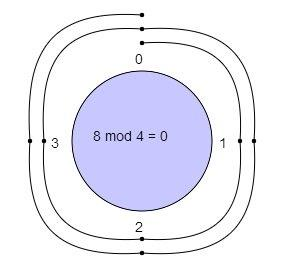
\includegraphics[width=.3\linewidth]{figures/mod8.jpg}
\end{frame}

\begin{frame}{Definition}
    $$-5 \bmod 3 = ?$$
    \centering
    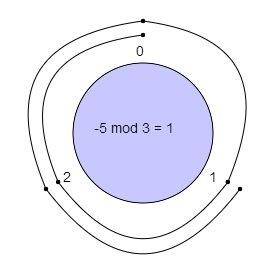
\includegraphics[width=.3\linewidth]{figures/mod-5.jpg}
\end{frame}

\begin{frame}{Definition}
    $$A \bmod B = (A + K \cdot B) \bmod B$$ 
    \\ For example:
    $$3  \bmod 10=3$$
    $$13 \bmod 10=3$$
    $$23 \bmod 10=3$$
    $$33 \bmod 10=3$$
\end{frame}

\begin{frame}{Congruence modulo}
Congruence modulo:
    $$A \equiv B \pmod C$$ 
\end{frame}

\begin{frame}{Congruence modulo}
    $$26 \equiv 11 \pmod 5$$ 
    \centering
    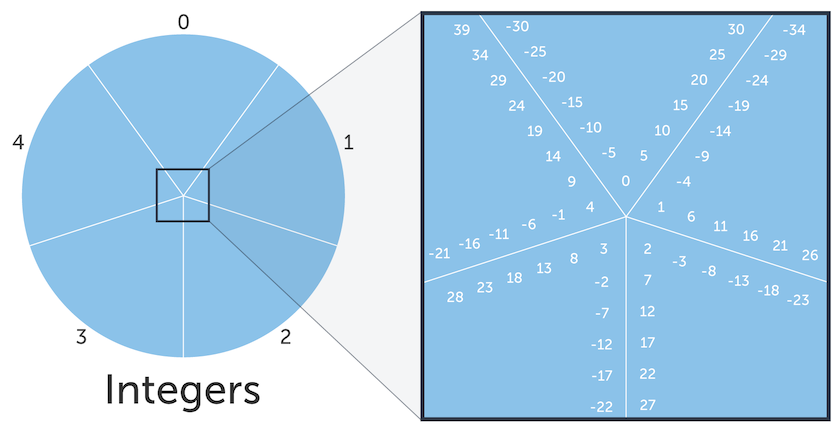
\includegraphics[width=.7\linewidth]{figures/congruent5.png}
\end{frame}

\begin{frame}{Congruence modulo}
    $$A \equiv B \pmod C$$ 
    \centering
    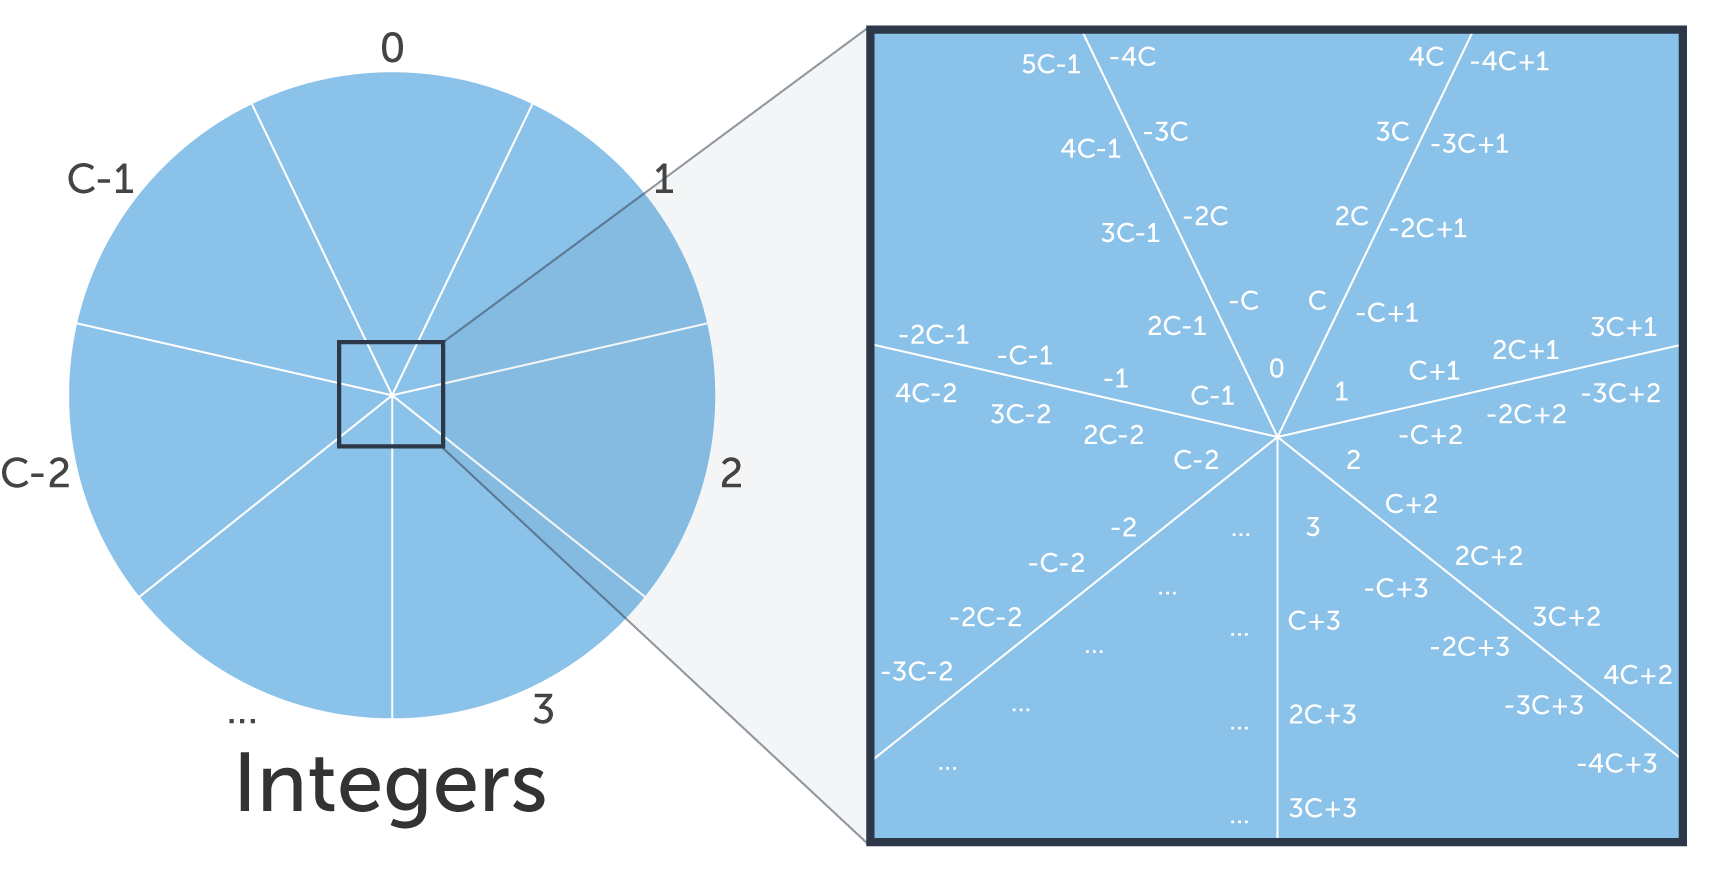
\includegraphics[width=.7\linewidth]{figures/congruentC.png}
\end{frame}

\begin{frame}{Equivalent Statements}
Equivalent Statements:
    \begin{itemize}
        \item $A \equiv B \pmod C$
        \item $A \bmod C = B \bmod C$
        \item $C \mid (A - B)$
        \item $A = B + K \cdot C$
    \end{itemize}
\end{frame}

\begin{frame}{Equivalent Statements}
For example:
    \begin{itemize}
        \item $13 \equiv 23 \pmod 5$
        \item $13 \bmod 5 = 23 \bmod 5$
        \item $5 \mid (13 - 23)$ by $5\times-2=-10$
        \item $13 = 23 + K \cdot 5$ by $K = -2$ 
    \end{itemize}
\end{frame}

\begin{frame}{Equivalence relation}
Equivalence relation:
    \begin{itemize}
        \item $A \equiv A \pmod C$ \textbf{[reflexive]}
        \item $A \equiv B \pmod C$ then $B \equiv A \pmod C$ \textbf{[symmetric]}
        \item $A \equiv B \pmod C$ and $B \equiv D \pmod C$ then $A \equiv D \pmod C$ \textbf{[transitive]}
    \end{itemize}
\end{frame}

\begin{frame}{Equivalence relation}
For example:
    \begin{itemize}
        \item $3 \equiv 3 \pmod 5$
        \item $3 \equiv 8 \pmod 5$ then $8 \equiv 3 \pmod 5$
        \item $3 \equiv 8 \pmod 5$ and if $8 \equiv 18 \pmod 5$ then $3 \equiv 18 \pmod 5$
    \end{itemize}
\end{frame}

\section{Addition and Subtraction}

\begin{frame}{The quotient remainder theorem}
Given any integer $A$, and a \textbf{positive} integer $B$, there exist unique integers $Q$ and $R$ such that:
    $$A= B * Q + R\ where\ 0 \leq R < B$$ 
If we can write a number in this form then 
    $$A \bmod B = R$$
\end{frame}


\begin{frame}{Webography}
  \begin{enumerate}
    \item Khan Academy - Journey into Cryptography \\ \url{https://tinyurl.com/jvqfq8t}
    \item \url{https://tinyurl.com/y7jbfqfe}
  \end{enumerate}
\end{frame}

%\begin{frame}{Applications}
%  Visual mining of cyclone paths.
%  \centering
%  \includegraphics[width=.85\linewidth]{Figures/cyclones.png}
%  \blfootnote{\tiny \href{https://tinyurl.com/nhmwerr}{(Turdukulov, IJGIS'14)}}
%\end{frame}

\
\end{document}
